\documentclass[border=4pt]{standalone}

\usepackage{amsmath}
\usepackage{tikz}
\usepackage{mathdots}
\usepackage{yhmath}
\usepackage{cancel}
\usepackage{color}
\usepackage{siunitx}
\usepackage{array}
\usepackage{multirow}
\usepackage{amssymb}
\usepackage{gensymb}
\usepackage{tabularx}
\usepackage{booktabs}
\usetikzlibrary{fadings}
\usetikzlibrary{patterns}


\begin{document}
 
 


\tikzset{every picture/.style={line width=0.75pt}} %set default line width to 0.75pt        

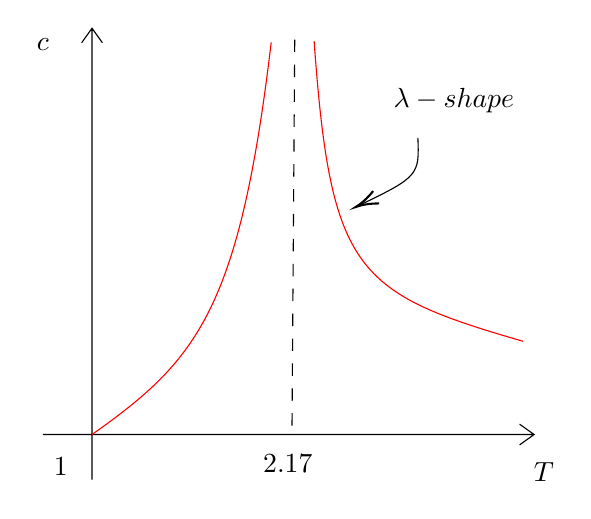
\begin{tikzpicture}[x=0.75pt,y=0.75pt,yscale=-1,xscale=1]
%uncomment if require: \path (0,413); %set diagram left start at 0, and has height of 413

%Shape: Axis 2D [id:dp8343884297871038] 
\draw  (189.33,291.42) -- (426,291.42)(213,95.67) -- (213,313.17) (419,286.42) -- (426,291.42) -- (419,296.42) (208,102.67) -- (213,95.67) -- (218,102.67)  ;
%Straight Lines [id:da034798154115386115] 
\draw  [dash pattern={on 4.5pt off 4.5pt}]  (310.67,101.17) -- (309.33,290.67) ;


%Curve Lines [id:da7297854689795116] 
\draw [color={rgb, 255:red, 255; green, 0; blue, 0 }  ,draw opacity=1 ]   (320,101.83) .. controls (328,213.17) and (340,223.17) .. (420.67,246.5) ;


%Curve Lines [id:da6854761400256277] 
\draw [color={rgb, 255:red, 255; green, 0; blue, 0 }  ,draw opacity=1 ]   (299.33,102.5) .. controls (284,231.83) and (263.33,255.83) .. (213,291.42) ;


%Curve Lines [id:da38869254519970253] 
\draw    (370,148.5) .. controls (370.65,166.14) and (370.67,167.13) .. (341.8,180.97) ;
\draw [shift={(340,181.83)}, rotate = 334.44] [color={rgb, 255:red, 0; green, 0; blue, 0 }  ][line width=0.75]    (10.93,-3.29) .. controls (6.95,-1.4) and (3.31,-0.3) .. (0,0) .. controls (3.31,0.3) and (6.95,1.4) .. (10.93,3.29)   ;


% Text Node
\draw (189.33,103.33) node   {$c$};
% Text Node
\draw (430.67,309.33) node   {$T$};
% Text Node
\draw (198,306.67) node   {$1$};
% Text Node
\draw (307.33,305.33) node   {$2.17$};
% Text Node
\draw (387.33,130.33) node   {$\lambda -shape$};


\end{tikzpicture}

\end{document}
